\documentclass[a4paper, 11pt]{article}
\usepackage[utf8]{inputenc} 
\usepackage[T1]{fontenc}
\usepackage{graphicx}
\usepackage[french]{babel} 
\usepackage{multirow,multicol}
\usepackage{amsmath, amssymb, latexsym}
\usepackage{pstricks,pst-node,pst-coil,pst-grad,pst-plot}
\usepackage{epsfig,subfigure}
\usepackage[lined,boxed]{algorithm}
\usepackage{algorithmic}
\usepackage{rotate}
\usepackage{url}
\usepackage{hyperref}
\usepackage{setspace}

\newtheorem{definition}{Definition}
\newtheorem{example}{Example}
\newtheorem{proposition}{Proposition}
\newtheorem{proof}{Proof}

\title{Présentation d'un Manic'shooter}
\author{Nicolas.A - David.R - Théo.B} 


\begin{document}

\maketitle
\tableofcontents
\section{Manic Shooter}
\subsection{Présentation}

Présentation d'un Manic Shooter:
Manic shooter ou Shoot them up ou Shmup qui signifie littéralement "Descendez-les tous".
Un Manic shooter est un jeu ou le joueur doit diriger un personnage ou véhicule devant tuer un grand nombres d'ennemis à l'aide d'armes de plus en plus puissantes au fur et à mesure des niveaux, le personnages doit esquiver les tirs ou projectile ennemis.
Ce système de jeu est sorti en 1978 avec 
\href{http://dictionnaire.sensagent.leparisien.fr/Space%20Invaders/fr-fr/}{Space inverders}
 present dans les salles d'arcades de base c'est un jeu 2D il trouve son succès enfin des années 80 début 90 dès que le graphisme tri-dimensionnelle apparut, son succès disparut.

 \begin{figure*}[ht!]
 \centering
 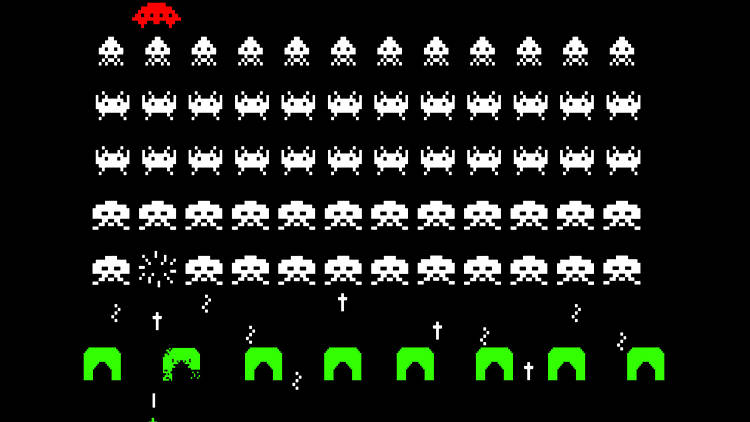
\includegraphics[width=0.7\linewidth]{space.jpg}
 \caption{Space inverders}
 \label{fig::example::one}
\end{figure*}

\subsection{diagramme}
diagramme 

\section{Cahier des charges}

\subsection{diagramme des besoins}

Le cahier des charges est l'une des chose essentiel pour bien débuter un projet sans cela la conception de notre logiciel serait devenue impossible.
Tout d'abord nous voulions définir les normes logique du manic shooter 
une carte / un personnage / des ennemies / ce déplacer / tirer etc ... 


 	\subsection{Une carte}
 	\begin{figure*}[ht!]
\centering
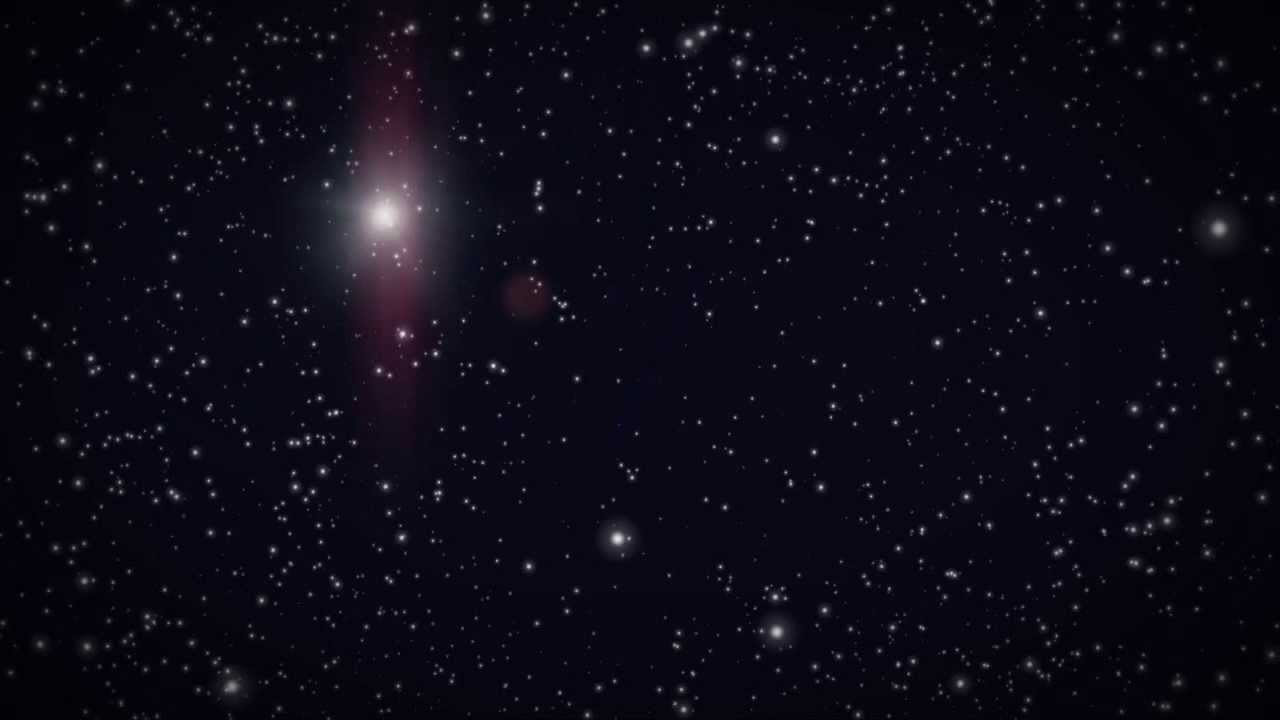
\includegraphics[width=0.8\linewidth]{Background.jpg}
\caption{Notre carte}
\end{figure*}
 	dans un premier temps il nous fallait une carte, c'est à dire un espace de jeu permettant a un héro d'être livrer à une épopée contre des ennemies,
 	notre premier réflexe à était de créer une grille et de créer un héro en l'initialisant en 1 et en initialisant des ennemies à 0 le reste de la grille étant que des "-", menant notre objectif jusqu'au bout nous nous sommes rendu compte qu'en associant l'interface graphique avec notre modèle de jeu posait problème et surtout qu'il existait une manière "plus simple" de faire la carte et surtout plus efficace, car en définissant la fenêtre avec Pygame cela aller être notre grille c'est à dire que la grille est la taille de fenêtre fois le nombre de pixels ce qui nous à simplifié la vie pour la suite.

 	
	\subsection{Un personnage}
un manic shooter à pour habitude d'avoir un héro qui ce déplace dans la carte, il nous fallait donc un héro ou personnage qui soit celui que le joueur va contrôler notre personnage :
\begin{figure*}[ht!]
\centering
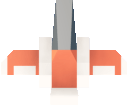
\includegraphics[width=0.1\linewidth]{spaceCraft1.png}
\caption{Notre personnage trouver sur internet "open source"}
\end{figure*}
ce personnage est équiper d'un réacteur qui le suit il à fallut intégrer cela au déplacement du héro et de faire en sorte que le réacteur soit collé au héro donc que la position soit identique .... suite .....

	\subsection{Des ennemis}
Le héro n'est pas le seul personnage à géré il nous faut également gérer les ennemies
	\subsection{Déplacement}
Une fois le contexte poser pour les personnages / la carte, c'est maintenant qu'intervient la notion de déplacement évidement le héro doit se déplacer pour éviter les ennemies et avant dans sont épopée, mais les ennemies doivent ce déplacer également, il ce déplace aléatoirement pour atteindre la héro pour cela nous allons utiliser la librairie random qui génère de chiffre aléatoire ce qui nous permet d'associer cela à des déplacement.
Au début les déplacement était de la "téléportation" c'est à dire que la position du héro était traité avec des rafraichissement d'images c'est à dire, quand le joueur appuie sur la touche déplacer le héro change de position et donc une nouvelle image et créer sur cette position et l'autre est supprimer, mais cela pose un problème, quand la vitesse du héro est trop grande on voit les différente images des différentes position du héro, ....... suite .......
	
	\subsection{Tir}
Généralement dans un manic shooter le héro doit posséder un tir qui va détruire les ennemies 
	\subsection{collisions}
Les personnages sont confronté à des collisions qui doivent être gérer, c'est à dire quand le tir va aller
\section{Choix des utilitaires utiliser}

le choix des utilitaires utilisés peut différer le rendu du projet nous avons donc dû tester au fur et à mesure ce qui aller nous convenir le mieux

\subsection{Tkinter}
tkinter est une interface graphique qui permet la conception de logiciel relativement pousser mais d'un rendu graphique faible, dans notre cas nous l'utilisons pour notre menu de notre jeu ce qui nous à rendement faciliter la tache car sur tkinter permet de créer des menu relativement facilement.
\subsection{Pygame}
Pygame est également une interface graphique qui est plus destiné au jeu,
dans notre cas nous l'utilisons pour l'intégralité de notre gameplay , les déplacement, les collisions , la carte et le choix de cette interface graphique nous est venu naturellement car elle offre une possibilité de déplacement intéressante.


\end{document}
